%\documentclass[a4paper, 12pt]{book}
\documentclass[oneside]{book}
\usepackage{index}
\usepackage{float}
\usepackage[english]{babel}
\usepackage[utf8x]{inputenc}
\usepackage{blindtext}
\usepackage{graphicx}
\usepackage{amsmath}
\usepackage{listings}
\usepackage[a4paper,bindingoffset=0.2in,%
            left=1in,right=1in,top=1in,bottom=1in,%
            footskip=.25in]{geometry}
\usepackage[font=LARGE]{caption}
\usepackage{cite}
\begin{document}
\begin{titlepage}
    \begin{center}
        \vspace*{1cm}
            
        \Huge
        \textbf{Creating Art with Deep Learning}
            
        \vspace{0.5cm}
        \LARGE
        \vspace{1.5cm}
            
        \textbf{Sanket Nagrale 185053}
        \hspace{8cm}
        \textbf{Shubhang Bhagat 185060}
        \hspace{8cm}
		\textbf{Abhishek Kapoor 185056}
        
            
        \vspace{0.8cm}
            
        \includegraphics[width=0.4\textwidth]{nith.png}
       
        \vspace{2cm}
        \LARGE
        Computer Science and Enginering

        NIT Hamirpur

		July 17, 2020
            
    \end{center}
\end{titlepage}
\chapter*{Abstract}
\section*{Neural Style Transfer}
\Large
Neural style transfer is an algorithm that combines the content of one image with the style of another image using CNN. Given a content image and a style image, the goal is to generate a target image that minimizes the content difference with the content image and the style difference with the style image.\cite{gatys2015neural}
\\
\\
The system uses neural representations to separate and recombine content and style of arbitrary images, providing a neural algorithm for the creation of artistic images.
\section*{What are Convolutional Neural Networks?}
\begin{figure}[h]
\centering
\includegraphics[width=1.0\textwidth]{Convolution Operation.png}
{\caption*{A Convolution Operation}}
\end{figure}
\pagebreak

A convolution is the simple application of a filter to an input that results in an activation. Repeated application of the same filter to an input results in a map of activations called a feature map, indicating the locations and strength of a detected feature in an input, such as an image.

A CNN algorithm can take an input image, extract learnable weights and biases to various objects in image and be able to tell from one another.
While the old methods required to be hand-engineered, with enough training, ConvNets learn the filters themselves. 


\begin{figure}[h]
\centering
\includegraphics[width=1.0\textwidth]{CNN.png}
\end{figure}


\section*{Transfer Learning}
One way to quickly get results (and often also get by with much less data) is to start not
from random initializations but from a network trained on some task with related data.
This is called transfer learning.
And we will selectively train some layers accordinig to our needs. This is called \emph{fine-tuning}.
Transfer learning has the benefit of decreasing the training time for a neural network model and can result in lower generalization error.
For this project, training a model from scratch will turn out to be an arduous task, hence we use pretrained models that come with Pytorch library.
\pagebreak
\section*{VGGNet}
\begin{figure}[h]
\centering
\includegraphics[scale=0.8]{VGG19.jpg}
{\caption*{VGGNet19 Architecture}}
\end{figure}
The VGG network architecture was introduced by Simonyan and Zisserman in their 2014 paper, \emph{Very Deep Convolutional Networks for Large Scale Image Recognition}.

This network is characterized by its simplicity, using only 3×3 convolutional layers stacked on top of each other in increasing depth. Reducing volume size is handled by max pooling. Two fully-connected layers, each with 4,096 nodes are then followed by a softmax classifier (above).\\

Torchvision has a pretrained VGG19 model. Pytorch provides access to a number of top-performing pre-trained models that were developed for image recognition tasks.
The first time a pre-trained model is loaded, Pytorch will download the required model weights, which may take some time given the speed of your internet connection.
\\
\textbf{Note:}
It is highly recommended to use cuda.
\chapter*{Code Explanation}
\section*{Loading the Libraries and Installing Requirements}
\begin{figure}[h]
\centering
\centerline{\includegraphics[scale=0.7]{loading.png}}
\end{figure}

The requirements to install the libraries are given in
requirements.txt file.

\textbf{Clone the github repository.}
\begin{lstlisting} 
git clone https://github.com/SankeNrale/Creating-Art-with
-Deep-Learning.git
\end{lstlisting}

\textbf{Install requirements} 
\begin{lstlisting} 
cd Creating-Art-with-Deep-Learning 
pip install -requirements.txt
\end{lstlisting}
\pagebreak
\section*{Preprocessing the Image}
\begin{figure}[h]
\centering
\centerline{\includegraphics[scale=0.69]{preprocessing.png}}
\end{figure}
Tensors are similar to NumPy’s ndarrays, with the addition being that Tensors can also be used on a GPU to accelerate computing.
\section*{Defining The Model}
\begin{figure}[h]
\centering
\centerline{\includegraphics[scale=0.69]{defining.png}}
\end{figure}
\begin{itemize}
\item \emph{self.select} chooses the layers to activate. 
\item \emph{self.VGG} selects the model VGG and \emph{pretrained=True} returns a pretrained model.
\end{itemize} 
\pagebreak
Pytorch has a unique way of defining the model.

In PyTorch, a model is represented by a regular Python class that inherits from the Module class.
The most fundamental methods it needs to implement are:\linebreak
\begin{itemize}
\item \_\_init\_\_(self)): it defines the parts that make up the model.

\item forward(self, x): it performs the actual computation, that is, it outputs a prediction, given the input x.
\end{itemize}

\section*{Training the Model}
\begin{figure}[H]
\centerline{\includegraphics[scale=.69]{1.png}}
\end{figure}
VGGNet was trained on ImageNet where images are normalized by mean=[0.485, 0.456, 0.406] and std=[0.229, 0.224, 0.225].
We use the same normalization statistics here.
Load content and style images with previously created load\_image function.
Make the style image same size as the content image.
We use the adam optimizer here. And we create a taget image using clone().
\begin{figure}[H]
\centerline{\includegraphics[scale=.69]{2.png}}
\end{figure}
view() basically reshapes the image in dimensions(c, h*w) where c is the number of the channels and h and w are height and width respectively.
torch.mm computes gram matrix which tells the correlation between the matrices.
content loss and style loss are calculated as given in the figure.
total loss is just a combination of both losses.
\begin{figure}[H]
\centerline{\includegraphics[scale=.84]{3.png}}
\end{figure}
The above code trains the model for a given number of epochs.
\pagebreak

\section*{Passing the Arguments}
\begin{figure}[H]
\centerline{\includegraphics[scale=.69]{argparse.png}}
\end{figure}

We can run our code using 
\begin{lstlisting}
python main.py --content png/content.png --style ;png/style.png
\end{lstlisting}
content.png and style.png should be in the png folder.

Important optional arguments are:
\begin{itemize}
\item total\_step: Number of Epochs
\item style\_weight: To change the amount of artistic style
\item lr: Learning rate
\end{itemize}

\LARGE
\section*{Results}
\begin{figure}[H]
\centerline{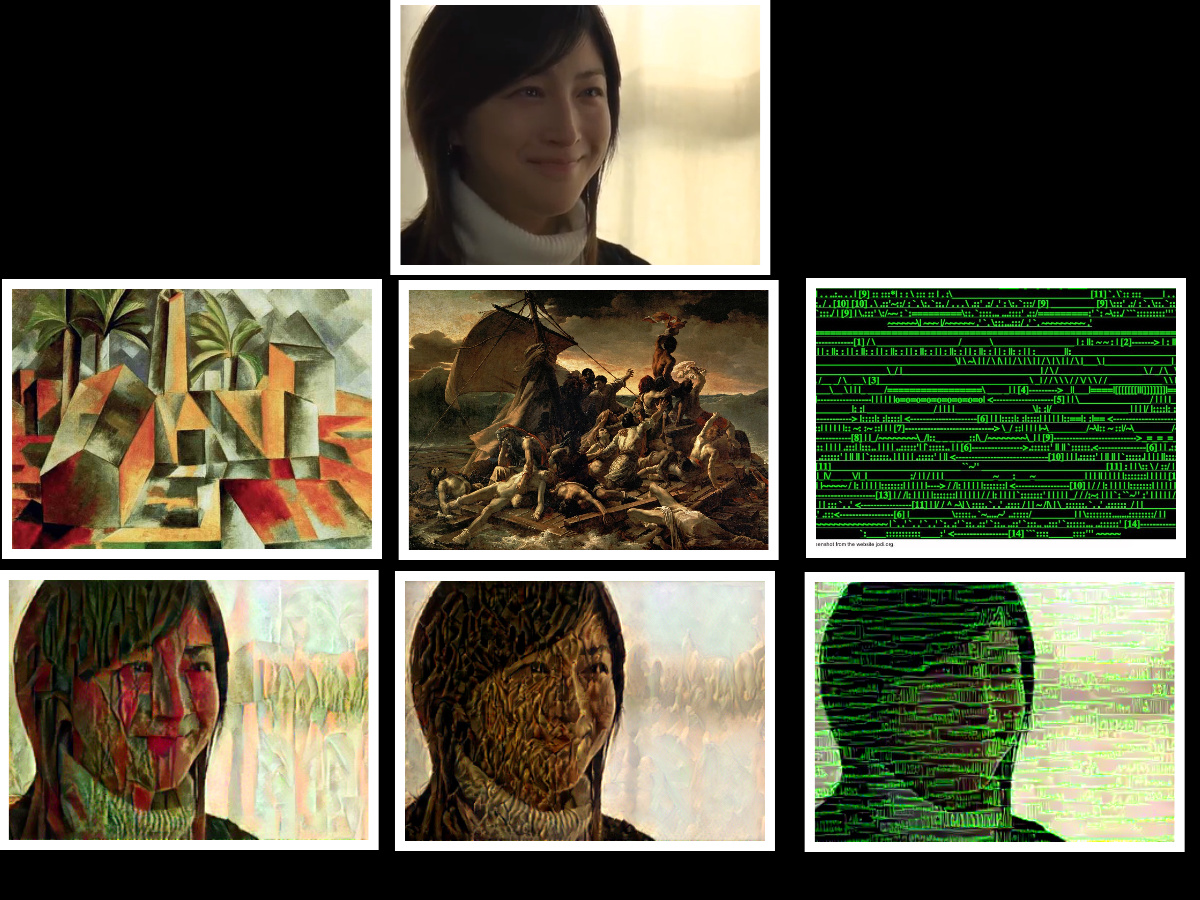
\includegraphics[scale=.5]{result.jpg}}
\end{figure}
\pagebreak

\bibliographystyle{plain}
\bibliography{reference1}
[2] https://towardsdatascience.com/neural-networks-             intuitions-2-dot-product-gram-matrix-and-neural-style-    transfer-5d39653e7916 
\bigbreak
\noindent[3] https://github.com/eriklindernoren/Fast-Neural-Style-Transfer
\bigbreak
\noindent[4] Coursera Deep Learning Specialization




\end{document}